%%
%% Time-stamp: <2019-05-08 01:01:17 stefan>
%%

\documentclass[swedish,10pt,a4paper]{article}

\usepackage[T1]{fontenc}
\usepackage[utf8]{inputenc}

% smallare marginal för anteckningar
%% \usepackage[marginparwidth=30pt]{geometry}

%%
%% använd Times istället för Computer Modern
\usepackage{mathptmx}
%% \usepackage{mathpazo}

\usepackage[swedish]{babel} %% babel
\usepackage{csquotes}       %% csquotes är för svenska beroende av babel

\usepackage[bottom]{footmisc} %% fotnötter i sidans nederkant

\usepackage{verbatim}         %% verbatim miljö

\usepackage{booktabs}         %% bottomrule/toprule !
\usepackage{xcolor}           %% \definecolor, den gråa bakgrunden i kodlistningarna
\definecolor{light-gray}{gray}{0.95}
%% \usepackage[flushleft]{threeparttable} %% fotnoter inuti tabellerna
\usepackage{hyperref}         %% hyperlänkar mellan text och bibliografin

%% \usepackage{footnote}

\usepackage{color}

%% \usepackage{tabularx}               %% mer användbara tabeller
\usepackage{tabu}                      %% mer användbara tabeller

\usepackage{listings} %% programkodslistningar
\lstset{basicstyle=\footnotesize,
  captionpos=b,
  backgroundcolor=\color{light-gray},
  extendedchars=true,
  breaklines=true,
  literate={ö}{{\"o}}1 {å}{{\aa}}1 {Å}{{\aA}}l {ä}{{\"a}}1 {Ö}{{\"O}}1 {Ä}{{\"A}}1
}

\usepackage{colortbl}

%\usepackage[fleqn]{mathtools}

%% PDF-inkludering
\usepackage{graphicx}
\usepackage{pst-pdf}

% \usepackage[fleqn]{mathtools}
% \usepackage{pgf}
% \newcommand{\BinaryAdd}[2]{%
% {#1}_2 + {#2}_2 = \pgfmathbin{0b#1 + 0b#2}% compute binary addition
% \pgfmathresult_2% format output to make it clear it is base 2
% }%

%% \usepackage[style=alphabetic,backend=biber]{biblatex}
\usepackage[style=authoryear,backend=biber]{biblatex} %%
\addbibresource[location=local]{bib.bib}
\addbibresource[location=local]{rfc.bib}
\addbibresource[location=local]{rfc_draft.bib}

\title{Labbrapport IT119G}
\author{Stefan Niskanen Skoglund\\IT119G\\19670927--5934}

\begin{document}

\maketitle

I arbetet har jag använt ett verktyg för systemadministration CFEngine
som ett stöd för korrekt inställning av isc:s DHCP:kontrollant
och deras DNS tjänst.
Dessutom används verktyget för att aktivera uppgraderingar av programvaran
förutom för pc01/pc02 på de virtuella maskinerna ns01,webserver01 och dhcp01.
Därav de extra två maskinerna cfengine och vcs \ref{network_organization} i ``server network''.
VCS:maskinen är värd för git som används av cfengine för att sina data.
Samma git:installation används även i rapportskrivningen.

% \includegraphics{network_diagram.tex}
%\includegraphics[height=200pt]{network_diagram_1.pdf}
%\includegraphics[width=\baselinewidth]{home_stefan_Skrivbord_IT119G_IT119G_labbrapport_network_diagram-job_176.pdf}
\begin{figure}
  \centering
  \caption{Labbnätverkets organisation}
  \label{network_organization}
  \fbox{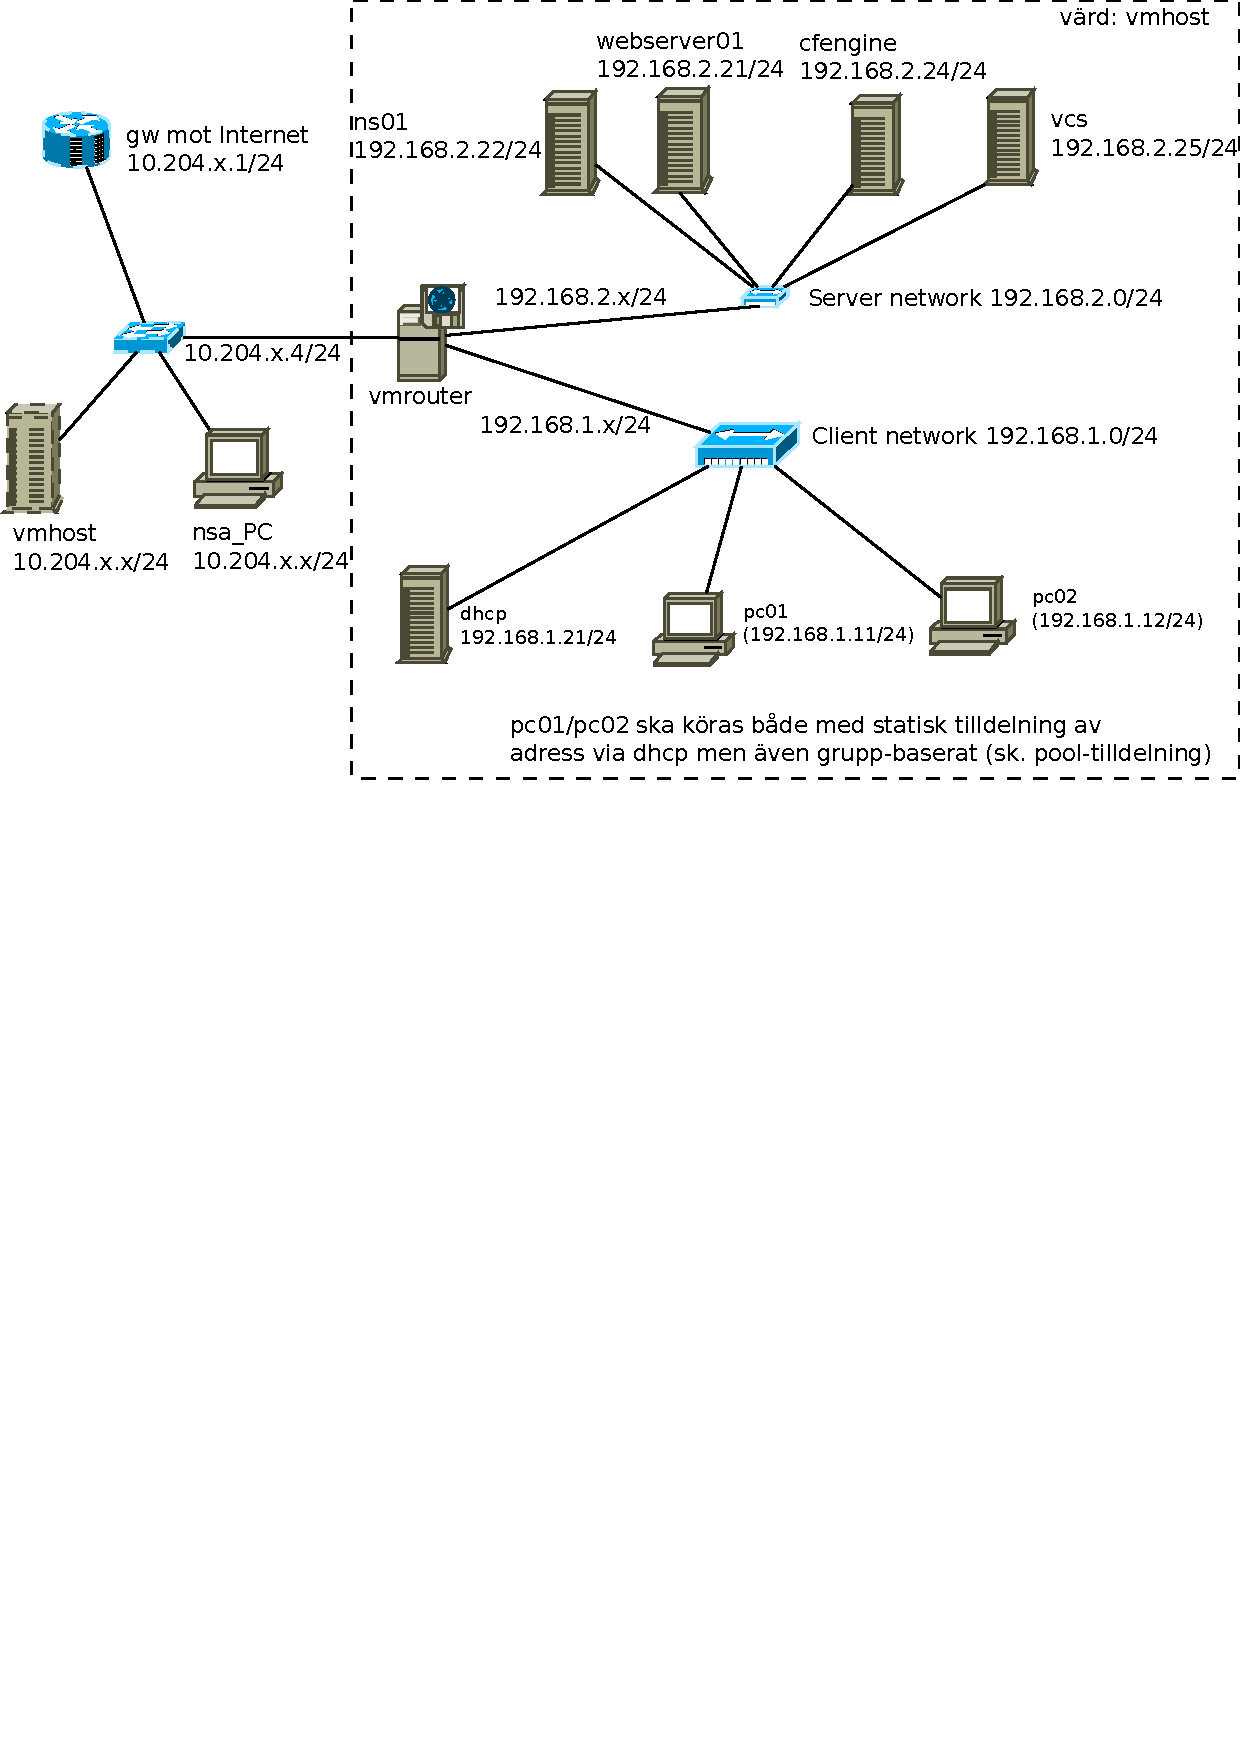
\includegraphics[width=\textwidth, clip, viewport=0 450 600 850 ]{network_diagram_export.pdf}}
\end{figure}

\section{Adressering i OSI:s länk-lager}\label{sec:adressering_i_osis_data_link_layer}

Ethernet utvecklades vid XEROX utvecklingscentrum i Palo-Alto\footcite[kapitel 1]{Spurgeon2000}
som ett svar på ett problem : nämligen hur XEROX nya uppfinning laserskrivaren
skulle kunna anslutas till den nya typen av datorer från XEROX där författare, tekniker,
ingenjörer och programmerare har kunnat fått sin egen maskin, XEROX ALTO.

Alto räknas som den första arbetsstationen i betydelsen en enanvändaredator med ett grafiskt
användaregränssnitt, en stor katodstråleskärm, ett roternade skivminne
och Doug Engelbarts pekdon, en mus.

Robert Metcalfe anställdes vid PARC 1972 bland annat på grund av sina erfarenheter av ARPANET
med avsikten att han skulle forska inom XEROX kontorsautomatiseringsprojekt.
Metcalfes Ethernet patenterades 1974 med avsikten att det skulle vara en viktig
komponent i XEROX produkter för kontoret.

Metcalfe blev 1977--1978 frustrerad av XEROX oförmåga att bygga och sälja produkter som
med den nya tekniken och att XEROX:s inställning till den var proprietär, ingen
annan skulle få använda den i sin produkt.

Metcalfe lämnade i slutet av 1978 XEROX med avsikten att i samarbete med andra
företag övertala XEROX att acceptera att Ethernet skulle standardiseras
och därmed bli tillgängligt som tillbehör till andra datorer än de från
XEROX. Intel, Digital Equipment och XEROX bildade DIX:konsortiet som
standardiserade Ethernet som IEEE 802.3 10base5.

\blockquote[\cite{Robert Metcalfe}]{I came to work one day at MIT and the computer had
  been stolen so I called DEC to break the news to them that this \$30,000
  computer that they'd lent me was gone. They thought this was the greatest thing that ever
  happened because it turns out I had in my possession the first computer small enough to be stolen!}

Digital Equipment hade målsättningen att till skillnad mot den äldre IMP:lösningen
kunna integrera anslutningen mot andra datornät inuti sina egna maskiner.
andra ndatornätsanslutningen inuti deras datorer.


\section{Adressöversättning i IP:baserade nätverk}\label{sec:address_translation}

Vilket protokoll används i ett nätverk där datorer vill översätta IPv4:s logiska adresser till något
som hårdvaran kan hantera? ARP = address resolution protocol.

RFC826 \footcite{rfc826} beskriver motivationen bakom och de tidiga orsakerna till ARP:s
utveckling. En viktig detalj i ARP är det faktum att det från
början utvecklades för DIX men tidigt generaliserades för att stödja
andra nätverkstekniker än DIX. DIX kom att standardiseras som IEEE 802.3 10Base5.

Generaliteten i ARP innebär att protokollet inte behövde förändras
när Ethernet bytte överföringsteknologi från en bussorienterad överföring
som i grunden fungerar som radiovågor till dagens stjärnformade nät där individuella datorer är
direkt anslutna till en för den reserverad anslutning i en sk.\ växel, anser jag.

% En växel är speciellt konstruerad för att vidarebefordra trafik från flera datorer antingen
% till dator som är ansluten i samma växel eller vidare via andra liknanden enheter till
% avsedd mottagare.

\subsection{översättning av IP-adress till de motsvarande MAC:adresserna}\label{trans_ip_mac}

\newcolumntype{s}{>{\columncolor[gray]{0.95}} p{4cm}}

\begin{table}
  \centering
  \caption{maskinnamn \& MAC-adresser}
  \begin{tabular}{|ss|}
    \bottomrule
    maskinnamn         & MAC-adress        \\
    ESXi (vmnic0)      & 6c:0b:84:08:fa:79 \\
    PC01 (e160)        & 00:50:56:36:16:67 \\ %% \footnote{Statisk tilldelning via gui}\\
    webserver01 (e160) & 00:0c:29:4a:cc:d2 \\ %% \footnote{automatiskt tilldelad adress i ESXi}\\
    \toprule
  \end{tabular}
\end{table}

MAC-adressen för PC01 och webserver01 gäller för virtuella nätanslutningar som
definieras av ESXi och tilldelas till virtuella maskiner i den värden
men de skiljer sig från vilken OUI som de tillhör.

\subsubsection{OUI = Organizationally Unique Identifier}
\label{subsubsec:oui}

OUI\footcite{rfc5342} är definierat som de första 24 binära bitarna av en adress dvs första
hälften av en adress.

Det är det sätt som adresser i MAC:systemet fördelas mellan ansvariga användare
där de fritt kan välja de 24 lägre bitarna i adressen.

En datorleverantör ger sina tillverkade maskiner en individuellt MAC:adress genom
ett 24 bitar långt serienummer som konkateneras med sin OUI.\@ IANA använder
sina egna OUI exempelvis som prefix i samband med IP:s gruppsändningsprotokoll men även
som ett sätt för en protokollansvariga organisation exv en programleverantör
som vill konstruera ett proprieärt protokoll dess egen adressrymd. Utökningarna i
ppp \footcite{rfc2153} är ett exempel på ett detta.


Vad kan man säga om vem som är leverantör av en maskin om man studerar en MAC:adress i ARP:tabellen?

% \begin{tablenotes}
% \item [1] Lenovo PC
% \item [2] Hewlett-Packard växel? Anslutning i gateway:maskin för gruppen 10.204.20.0
% \item [3] Hewlett-Packard växel? Anslutning i gateway:maskin för gruppen 10.204.8.0
% \item [4] Har använt mer än en datorgrupp
% \end{tablenotes}

MAC-adresser i klassisk Ethernet som även är känt som DIX:standarden efter
de bakomliggande leverantörerna fördelar användbara adresser genom att tilldela
leverantörerna ett eller flera prefix eller adressområden som de blev ansvarig för. MAC-adressen är 48 bitar lång
och prefixet är hälften av det dvs 24 bitar. Leverantören använder
de 24 övriga bitarna för att differentiera mellan maskiner men även anslutningskort för ethernet.

Många prefix reserverades från första början för olika användningar. Ett exempel på
sådan användning är multicast i IP:nätverk där adressen 224.20.20.2 nominerar
de maskiner som är medlemmar av en viss grupp.

Varför syns det inte någon förändring i ARP-tabellen efter att
ha försökt ping:a specifik maskin bortanför utgående anslutning ?
PC01 har i ARP:tabellen lagt till VMrouter:maskinens MAC-adress.

\section{Trafikspårning}
\label{sec:wireshark_usage}

Vilket protokoll använder ping\footnote{se man -s 8 ping} ? ICMP:s echo:begäran (ICMP typ 8) och ICMP:s motsvarande svarspaket (ICMP typ 0.)

Eftersom trafik till andra maskiner än de fyra som är direkt åtkomliga i ``Client network'' skickas via
``VMrouter'' behövs enbart den maskinens MAC:adress i ARP:tabellen (arp funktionen i operativsystemet hanterar
next-hop:adresser.)\@10.204.20.1 är inte någon av dem.

\section{DHCP}
\label{sec:dhcp_konf}

Jag flyttade ``pc01'' till  ``Server network'' sedan klagade den maskinen på ``jag är bortkopplad !''.
Dessutom fick den inte någon ny IP:adress eftersom det inte finns någon ``DHCP'' tjänst i det nätet.

Däremot sänds det på det nätet ut ett antal ``DHCP Discover''.

Normalt sett skickas ``broadcast'':paket (mottagaradress 255.255.255.255 med avsändare 0.0.0.0) till port 67 från port 68 med UDP från
den klient som vill ha en ny adress (``DHCP Request''). Dhcp:kontrollanten svarar med ett ``DHCP ACK'' från sin
egen IPv4:adress till klientens MAC-adress med klientens korrekta IPv4:adress och andra optioner som exempelvis
korrekt DNS:maskin och DNS:domännamn i samma paket.

\subsection{loggar}

``/var/lib/dhcp/dhcpd.leases'' innehåller uppgifter om vilka klienter som har fått
automatisk tilldelade adresser via ``range'':uppgiften. Om maskinen inte syns i leases och
har en statiskt tilldelad adress så är det fullt normalt - dpcpd.leases har inte
uppgifter om maskiner vars adresser är statiskt tilldelade
som exempelvis för pc01:

%% \definecolor{light-gray}{gray}{0.95}

% \lstset{basicstyle=\footnotesize,
% captionpos=b,
% backgroundcolor=\color{light-gray},
% extendedchars=true,
% breaklines=true,
% literate={ö}{{\"o}}1 {å}{{\aa}}1 {Å}{{\aA}}l {ä}{{\"a}}1 {Ö}{{\"O}}1 {Ä}{{\"A}}1
% }
%   \begin{lstlisting}[caption={/etc/dhcp/dhcpd.conf}]
%     host  pc01 {
%     hardware ethernet 00:50:56:36:16:67;
%     fixed-address 192.168.1.11;
%   }
%   \end{lstlisting}

%   \begin{lstlisting}[caption={/var/lib/dhcp/dhcpd.leases}]
%     lease 192.168.1.11 {
%     starts 5 2019/03/29 11:25:55;
%     ends 5 2019/03/29 11:35:55;
%     cltt 5 2019/03/29 11:25:55;
%     binding state active;
%     next binding state free;
%     rewind binding state free;
%     hardware ethernet 00:50:56:36:16:67;
%     client-hostname "pc01";
%   }
%   \end{lstlisting}

\section{broadcastdomäner}
\label{sec:broadcastdomains}

VMrouter borde vara ansluten till tre st (det lokala arbetsgruppsnätet, Server network och Client network.)

\section{DNS:konfiguration}
\label{sec:dns_konf}

% \begin{lstlisting}[caption={Några frågor, dig +search www}]
%   ; <<>> DiG 9.9.4-RedHat-9.9.4-73.el7_6 <<>> +search www
%   ;; global options: +cmd
%   ;; Got answer:
%   ;; ->>HEADER<<- opcode: QUERY, status: NOERROR, id: 63149
%   ;; flags: qr aa rd ra; QUERY: 1, ANSWER: 2, AUTHORITY: 1, ADDITIONAL: 2

%   ;; OPT PSEUDOSECTION:
%   ; EDNS: version: 0, flags:; udp: 4096
%   ;; QUESTION SECTION:
%   ;www.b18steni.it119g.nsa.his.se.	IN	A

%   ;; ANSWER SECTION:
%   www.b18steni.it119g.nsa.his.se.	10 IN	CNAME	webserver01.b18steni.it119g.nsa.his.se.
%   webserver01.b18steni.it119g.nsa.his.se.	10 IN A	192.168.2.21

%   ;; AUTHORITY SECTION:
%   b18steni.it119g.nsa.his.se. 10	IN	NS	ns01.b18steni.it119g.nsa.his.se.

%   ;; ADDITIONAL SECTION:
%   ns01.b18steni.it119g.nsa.his.se. 10 IN	A	192.168.2.22

%   ;; Query time: 0 msec
%   ;; SERVER: 192.168.2.22#53(192.168.2.22)
%   ;; WHEN: fre mar 29 13:32:30 CET 2019
%   ;; MSG SIZE  rcvd: 136
% \end{lstlisting}

% \begin{lstlisting}[caption={Några frågor, dig -t NS b18steni.it119g.nsa.his.se.}]
%   ; <<>> DiG 9.9.4-RedHat-9.9.4-73.el7_6 <<>> -t NS b18steni.it119g.nsa.his.se.
%   ;; global options: +cmd
%   ;; Got answer:
%   ;; ->>HEADER<<- opcode: QUERY, status: NOERROR, id: 20764
%   ;; flags: qr aa rd ra; QUERY: 1, ANSWER: 1, AUTHORITY: 0, ADDITIONAL: 2

%   ;; OPT PSEUDOSECTION:
%   ; EDNS: version: 0, flags:; udp: 4096
%   ;; QUESTION SECTION:
%   ;b18steni.it119g.nsa.his.se.	IN	NS

%   ;; ANSWER SECTION:
%   b18steni.it119g.nsa.his.se. 10	IN	NS	ns01.b18steni.it119g.nsa.his.se.

%   ;; ADDITIONAL SECTION:
%   ns01.b18steni.it119g.nsa.his.se. 10 IN	A	192.168.2.22

%   ;; Query time: 0 msec
%   ;; SERVER: 192.168.2.22#53(192.168.2.22)
%   ;; WHEN: fre mar 29 13:34:03 CET 2019
%   ;; MSG SIZE  rcvd: 90
% \end{lstlisting}

% \begin{lstlisting}[caption={Några frågor, dig -t A  ns01.b18steni.it119g.nsa.his.se.}]
%   ;; global options: +cmd
%   ;; Got answer:
%   ;; ->>HEADER<<- opcode: QUERY, status: NOERROR, id: 38195
%   ;; flags: qr aa rd ra; QUERY: 1, ANSWER: 1, AUTHORITY: 1, ADDITIONAL: 1

%   ;; OPT PSEUDOSECTION:
%   ; EDNS: version: 0, flags:; udp: 4096
%   ;; QUESTION SECTION:
%   ;ns01.b18steni.it119g.nsa.his.se. IN	A

%   ;; ANSWER SECTION:
%   ns01.b18steni.it119g.nsa.his.se. 10 IN	A	192.168.2.22

%   ;; AUTHORITY SECTION:
%   b18steni.it119g.nsa.his.se. 10	IN	NS	ns01.b18steni.it119g.nsa.his.se.

%   ;; Query time: 0 msec
%   ;; SERVER: 192.168.2.22#53(192.168.2.22)
%   ;; WHEN: fre mar 29 13:35:29 CET 2019
%   ;; MSG SIZE  rcvd: 90
% \end{lstlisting}

% \begin{lstlisting}[caption={Några frågor, dig -t SOA @ns1.google.com. google.com.}]
%   ;; Got answer:
%   ;; ->>HEADER<<- opcode: QUERY, status: NOERROR, id: 24539
%   ;; flags: qr aa rd; QUERY: 1, ANSWER: 1, AUTHORITY: 4, ADDITIONAL: 9
%   ;; WARNING: recursion requested but not available

%   ;; OPT PSEUDOSECTION:
%   ; EDNS: version: 0, flags:; udp: 512
%   ;; QUESTION SECTION:
%   ;google.com.			IN	SOA

%   ;; ANSWER SECTION:
%   google.com.		60	IN	SOA	ns1.google.com. dns-admin.google.com. 240952484 900 900 1800 60

%   ;; AUTHORITY SECTION:
%   google.com.		345600	IN	NS	ns2.google.com.
%   google.com.		345600	IN	NS	ns4.google.com.
%   google.com.		345600	IN	NS	ns1.google.com.
%   google.com.		345600	IN	NS	ns3.google.com.

%   ;; ADDITIONAL SECTION:
%   ns2.google.com.		345600	IN	A	216.239.34.10
%   ns2.google.com.		345600	IN	AAAA	2001:4860:4802:34::a
%   ns4.google.com.		345600	IN	A	216.239.38.10
%   ns4.google.com.		345600	IN	AAAA	2001:4860:4802:38::a
%   ns1.google.com.		345600	IN	A	216.239.32.10
%   ns1.google.com.		345600	IN	AAAA	2001:4860:4802:32::a
%   ns3.google.com.		345600	IN	A	216.239.36.10
%   ns3.google.com.		345600	IN	AAAA	2001:4860:4802:36::a

%   ;; Query time: 25 msec
%   ;; SERVER: 216.239.32.10#53(216.239.32.10)
%   ;; WHEN: fre mar 29 13:37:10 CET 2019
%   ;; MSG SIZE  rcvd: 333
% \end{lstlisting}

% \begin{lstlisting}[caption={Några frågor, 'dig -t A www' med eller utan '+search'}]
%   dig +search www

%   ; <<>> DiG 9.10.3-P4-Ubuntu <<>> +search www
%   ;; global options: +cmd
%   ;; Got answer:
%   ;; ->>HEADER<<- opcode: QUERY, status: NOERROR, id: 61521
%   ;; flags: qr aa rd ra; QUERY: 1, ANSWER: 2, AUTHORITY: 1, ADDITIONAL: 2

%   ;; OPT PSEUDOSECTION:
%   ; EDNS: version: 0, flags:; udp: 4096
%   ;; QUESTION SECTION:
%   ;www.b18steni.it119g.nsa.his.se.	IN	A

%   ;; ANSWER SECTION:
%   www.b18steni.it119g.nsa.his.se.	10 IN	CNAME	webserver01.b18steni.it119g.nsa.his.se.
%   webserver01.b18steni.it119g.nsa.his.se.	10 IN A	192.168.2.21

%   ;; AUTHORITY SECTION:
%   b18steni.it119g.nsa.his.se. 10	IN	NS	ns01.b18steni.it119g.nsa.his.se.

%   ;; ADDITIONAL SECTION:
%   ns01.b18steni.it119g.nsa.his.se. 10 IN	A	192.168.2.22

%   ;; Query time: 0 msec
%   ;; SERVER: 192.168.2.22#53(192.168.2.22)
%   ;; WHEN: Fri Mar 29 13:42:24 CET 2019
%   ;; MSG SIZE  rcvd: 136

%   dig www

%   ; <<>> DiG 9.10.3-P4-Ubuntu <<>> www
%   ;; global options: +cmd
%   ;; Got answer:
%   ;; ->>HEADER<<- opcode: QUERY, status: NXDOMAIN, id: 44523
%   ;; flags: qr rd ra ad; QUERY: 1, ANSWER: 0, AUTHORITY: 1, ADDITIONAL: 1

%   ;; OPT PSEUDOSECTION:
%   ; EDNS: version: 0, flags:; udp: 4096
%   ;; QUESTION SECTION:
%   ;www.				IN	A

%   ;; AUTHORITY SECTION:
%   .			10692	IN	SOA	a.root-servers.net. nstld.verisign-grs.com. 2019032900 1800 900 604800 86400

%   ;; Query time: 2 msec
%   ;; SERVER: 192.168.2.22#53(192.168.2.22)
%   ;; WHEN: Fri Mar 29 13:42:33 CET 2019
%   ;; MSG SIZE  rcvd: 107
% \end{lstlisting}

\subsection{Betydelsen av punkt eller inte i frågor med dig}

Dig:programmet kan använda den sökdomän i DNS som maskinerna är konfigurerade för, ``b18steni.it119g.nsa.his.se'' i mitt fall och ``xxxx.it119g.nsa.his.se''
för övriga klasskamrater.
Dock kräver ``dig'' att flaggan ``+search'' specificeras då eller att användaren självt specificerar domännamnet.

De här frågorna är ekvivalenta:
\begin{verbatim}
dig www.
dig www
\end{verbatim}
och dessa:
\begin{verbatim}
dig www.b18steni.it119g.nsa.his.se.
dig +search www
\end{verbatim}

\section{DNS:konfiguration}\label{sec:dns_config}

\section{WEB:tjänst}\label{sec:httpd_config}

DNS i ns01 får frågan:
Jag vill få en A:uppgift för maskinen ``webserver01.b18steni.it119g.nsa.his.se''.
Har du någrar data om detta ?
BIND:programmet svarar med motsvarande A:uppgift dvs vad ``webserver01.b18steni.it119g.nsa.his.se''
heter och vilken IP:adress den har.

---
; <<>> DiG 9.10.3-P4-Ubuntu <<>> @192.168.2.22 webserver01.b18steni.it119g.nsa.his.se
; (1 server found)
;; global options: +cmd
;; Got answer:
;; ->>HEADER<<- opcode: QUERY, status: NOERROR, id: 9893
;; flags: qr aa rd; QUERY: 1, ANSWER: 1, AUTHORITY: 1, ADDITIONAL: 2
;; WARNING: recursion requested but not available

;; OPT PSEUDOSECTION:
; EDNS: version: 0, flags:; udp: 4096
;; QUESTION SECTION:
;webserver01.b18steni.it119g.nsa.his.se.	IN A

;; ANSWER SECTION:
webserver01.b18steni.it119g.nsa.his.se.	10 IN A	192.168.2.21

;; AUTHORITY SECTION:
b18steni.it119g.nsa.his.se. 10	IN	NS	ns01.b18steni.it119g.nsa.his.se.

;; ADDITIONAL SECTION:
ns01.b18steni.it119g.nsa.his.se. 10 IN	A	192.168.2.22

;; Query time: 0 msec
;; SERVER: 192.168.2.22\#53(192.168.2.22)
;; WHEN: Sun Apr 14 17:02:20 CEST 2019
;; MSG SIZE  rcvd: 118
---
Det protokoll från applikationsnivån som används är DNS (eller domain.)
Transportprotokollet för sådana här frågor är vanligtvis UDP med det
undantaget att vissa frågor pga svaren blir för stora för ett UDP:paket
sänds med TCP. Min DNS:tjänst i ns01 dvs 192.168.2.22.
Avsändningsporten är 53683 och mottagande 53 (klienten.)
Från klienten ser det ut som att svaret kommer från port 53 destinerat
till 53683.


\section{Uppgifter --- statisk IP:adressering}\label{sec:statisk_ip_adressering}

\begin{table}
  \centering
  \caption{maskinnamn, MAC-adresser och leverantör}
  \begin{tabular}{|sss|}
    \bottomrule
    maskinnamn         & MAC-adress        & Ansvarig leverantör\\
    ESXi (vmnic0)      & 6c:0b:84:08:fa:79 & Universal Global Scientific Industrial Co.,Ltd.\\
    PC01 (e160)        & 00:50:56:36:16:67 & VMware Inc\\
    webserver01 (e160) & 00:0c:29:4a:cc:d2 & VMware Inc\\
    dhcp01 (e160)      & 00:0c:29:9e:43:6a & VMware Inc\\
    10.204.20.1        & bc:ea:fa:11:94:33 & Hewlett-Packard\\
    10.204.8.1         & bc:ea:fa:11:94:47 & Hewlett-Packard\\
    \toprule
  \end{tabular}
\end{table}


\section{TCP-anslutningsfaser för en HTTP:överföring }\label{sec:tcp_phases_http}

TCP definieras som en strömbaserad tillförlitlig förbindelse där strömbaserad ska ses som
att förbindelsen ses som ett flöde utan några för applikationen direkt synliga gränser.

TCP är tillförlig i betydelsen att avsändare och mottagare ska meddelas om rapport det blir
ett avbrott i förbindelsen som medför att det hos mottagaren saknas data.
Data som leveraras till mottagande program får ävenså inte vara förvanskat och alla data ska överlämnas
i samma ordning som när det överlämnades av avsändande program till sin maskins TCP:modul.

TCP:modul ska ses som den del av operativsystem eller det användareprogram som implementerar TCP (och
underliggande moduler exv IP och ARP.) DECnet är ett exempel där användaren har installerat ett
separat program för att implementera TCP ovanför en otillförlitlig transport via IP, DECnet eller X25.

Tre-stegs handskakning
\begin{verbatim}
--
SYN
SYN+ACK
ACK
--
\end{verbatim}

\appendix

I systemet modifierade filer inklusive DNS zoner.
Egentligen konfiguration av bind\footnote{se ``man -s 8 bind''} självt.

\section{DNS}\label{sec:appendix_bind_config}

\begin{lstlisting}[caption={/etc/bind/named.conf}]
  //
  // avsedd för ns01.b18steni.it119g.nsa.his.se
  //
  // cfe-regler från 192.168.2.24
  // senast uppdatering av policy:
  //

  include "/etc/bind/named.conf.options";
  include "/etc/bind/named.conf.local";
\end{lstlisting}

\begin{lstlisting}[caption={/etc/bind/named.conf.local}]
  //
  // avsedd för ns01.b18steni.it119g.nsa.his.se
  //
  // cfe-regler från 192.168.2.24
  // senast uppdatering av policy:
  //

  zone "b18steni.it119g.nsa.his.se" {
    type master;
    file "/etc/bind/zones/db.b18steni";
  };

  zone "168.192.in-addr.arpa" {
    type master;
    file "/etc/bind/zones/db.b18steni_192_rev";
  };
\end{lstlisting}

\begin{lstlisting}[caption={/etc/bind/named.conf.options}]
  //
  // avsedd för ns01.b18steni.it119g.nsa.his.se
  //
  // cfe-regler från 192.168.2.24
  // senast uppdatering av policy:
  //

  acl my_computers { 192.168.0.0/16; 10.204.12.0/24; 10.204.20.0/24; };

  options {
    directory "/var/cache/bind";
    dnssec-validation auto;

    forwarders {
      10.0.252.201;
      10.0.252.202;
    };

    listen-on-v6 { any; };
    auth-nxdomain no;    \# conform to RFC1035

    allow-recursion { my_computers; };
    allow-query { any; };
  };
\end{lstlisting}

\section{DNS zoner}\label{sec:appendix_dns_zones}

\texttt{db.b18steni.it119g.nsa.his.se} och motsvarande baklängesmapp\@
\texttt{ db.192.168.2/db.192.168.1} för trädet \texttt{2.168.192.in-addr.arpa}
och \texttt{1.168.192.in-addr.arpa}.

\section{isc dhcp}\label{sec:appendix_isc_dhcpd_config}

\begin{lstlisting}[caption={/etc/dhcp/dhcpd.conf} (pool-baserad allokering av adresser)]
#
# avsedd för dhcp01.b18steni.it119g.nsa.his.se
#
# def.json tidsstämpel: Time-stamp: <2019-05-06 12:09:15 nsa>
# host.json tidsstämpel: Time-stamp: <2019-03-29 13:17:21 nsa>
# senast uppdatering av policy: Mon May  6 12:13:17 2019
#
# cfe-regler från 192.168.2.24
#

ddns-update-style none;

option routers 192.168.1.1;
option domain-name "b18steni.it119g.nsa.his.se";
option domain-name-servers 192.168.2.22;

option ntp-servers 194.58.203.20;
default-lease-time 600;
max-lease-time 7200;

# If this DHCP server is the official DHCP server for the local
# network, the authoritative directive should be uncommented.
authoritative;

# Use this to send dhcp log messages to a different log file (you also
# have to hack syslog.conf to complete the redirection).
log-facility local7;


#
# utan static_dhcp_mapping
#
subnet 192.168.1.0 netmask 255.255.255.0 {
  range 192.168.1.10 192.168.1.20;
  option routers 192.168.1.1;
}
\end{lstlisting}
\newpage
\begin{lstlisting}[caption={/etc/dhcp/dhcpd.conf} (statisk allokering av adresser)]
#
# avsedd för dhcp01.b18steni.it119g.nsa.his.se
#
# def.json tidsstämpel: Time-stamp: <2019-05-06 12:09:15 nsa>
# host.json tidsstämpel: Time-stamp: <2019-03-29 13:17:21 nsa>
# senast uppdatering av policy: Mon May  6 12:13:17 2019
#
# cfe-regler från 192.168.2.24
#

ddns-update-style none;

option routers 192.168.1.1;
option domain-name "b18steni.it119g.nsa.his.se";
option domain-name-servers 192.168.2.22;

option ntp-servers 194.58.203.20;
default-lease-time 600;
max-lease-time 7200;

# If this DHCP server is the official DHCP server for the local
# network, the authoritative directive should be uncommented.
authoritative;

# Use this to send dhcp log messages to a different log file (you also
# have to hack syslog.conf to complete the redirection).
log-facility local7;


#
# utan static_dhcp_mapping
#
subnet 192.168.1.0 netmask 255.255.255.0 {
  range 192.168.1.10 192.168.1.20;
  option routers 192.168.1.1;
}
\end{lstlisting}

\begin{lstlisting}[caption={/var/lib/dhcp/dhcpd.leases}]
lease 192.168.1.11 {
  starts 5 2019/03/29 11:25:55;
  ends 5 2019/03/29 11:35:55;
  cltt 5 2019/03/29 11:25:55;
  binding state active;
  next binding state free;
  rewind binding state free;
  hardware ethernet 00:50:56:36:16:67;
  client-hostname "pc01";
}
\end{lstlisting}

\printbibliography{}
\end{document}
